% ============================================================================
% Lecture 18 (B17): PINNs I --- Residual Learning for ODEs and PDEs
% Deep Learning for Solving and Estimating Dynamic Models in Economics and Finance
% Course author: Simon Scheidegger
% ============================================================================

\documentclass[aspectratio=169,11pt]{beamer}

% ---------- Theme and colors ----------
\usecolortheme{dove}
\setbeamertemplate{navigation symbols}{}
\setbeamertemplate{footline}{%
  \hfill\usebeamerfont{page number in head/foot}%
  \usebeamercolor[fg]{normal text}%
  \insertframenumber\,/\,\inserttotalframenumber\kern1em\vskip4pt}
\setbeamerfont{frametitle}{size=\huge}

% ---------- Packages ----------
\usepackage[utf8]{inputenc}
\usepackage[T1]{fontenc}
\usepackage{amsmath,amssymb,amsfonts}
\usepackage{bm}
\usepackage{graphicx}
\usepackage{tikz}
\usetikzlibrary{shapes,arrows.meta,positioning,calc,fit,backgrounds,patterns,decorations.pathreplacing}
\usepackage{pgfplots}
\pgfplotsset{compat=1.18}
\usepackage{booktabs}
\usepackage{hyperref}
\usepackage{multicol}
\usepackage{xcolor}
\usepackage{algorithm}
\usepackage{algorithmic}
\usepackage{listings}

% ---------- Listings style for Python ----------
\lstset{
    language=Python,
    basicstyle=\small\ttfamily,
    keywordstyle=\color{uzhblue}\bfseries,
    commentstyle=\color{uzhgreydark}\itshape,
    stringstyle=\color{darkgreen},
    showstringspaces=false,
    breaklines=true,
    breakatwhitespace=true,
    columns=fullflexible,
    frame=none,
    xleftmargin=0pt,
    aboveskip=4pt,
    belowskip=4pt,
    escapeinside={(*@}{@*)},
}

% ---------- Custom colors ----------
\definecolor{uzhblue}{rgb}{0,0,0.5}
\definecolor{uzhgreylight}{RGB}{236,238,241}
\definecolor{uzhgreydark}{RGB}{81,86,94}
\definecolor{harvardcrimson}{RGB}{153,0,0}
\definecolor{unil@blue}{RGB}{0,140,204}
\definecolor{unil@black}{RGB}{35,31,32}
\definecolor{darkgreen}{RGB}{0,100,0}
\definecolor{darkred}{RGB}{139,0,0}
\definecolor{softblue}{RGB}{70,130,180}
\definecolor{softorange}{RGB}{230,159,0}
\definecolor{softgreen}{RGB}{0,158,115}

% ---------- Set beamer colors ----------
\setbeamercolor{frametitle}{bg=uzhgreylight, fg=uzhblue}
\setbeamercolor{title}{fg=uzhblue}
\setbeamercolor{structure}{fg=uzhblue}
\setbeamercolor{block title}{bg=unil@blue, fg=white}
\setbeamercolor{block body}{bg=uzhgreylight}
\setbeamercolor{block title alerted}{bg=darkred,fg=white}
\setbeamercolor{block body alerted}{bg=red!5}
\setbeamercolor{block title example}{bg=darkgreen,fg=white}
\setbeamercolor{block body example}{bg=green!5}
\setbeamercolor{item}{fg=unil@black}
\setbeamercolor{normal text}{fg=unil@black}

% ---------- Emphasis and hyperlinks ----------
\newcommand{\emphc}[1]{\textcolor{harvardcrimson}{#1}}
\hypersetup{colorlinks,linkcolor=harvardcrimson,urlcolor=harvardcrimson}

% ---------- Math commands ----------
\newcommand{\x}{\bm{x}}
\newcommand{\w}{\bm{w}}
\newcommand{\bb}{\bm{b}}
\newcommand{\z}{\bm{z}}
\newcommand{\W}{\bm{W}}
\newcommand{\X}{\bm{X}}
\renewcommand{\a}{\bm{a}}
\newcommand{\R}{\mathbb{R}}
\newcommand{\E}[1]{\mathbb{E}\!\left[#1\right]}
\DeclareMathOperator*{\argmin}{arg\,min}
\DeclareMathOperator*{\argmax}{arg\,max}

% ---------- Title ----------
\title[Lecture 19 (B18)]{Lecture 19 (B18): PINNs for Economic PDEs --- Boundary Conditions, HJB, Black--Scholes}
\subtitle{Soft vs hard BCs, HJB cake-eating, DGM architecture, Black--Scholes pricing}
\author{Simon Scheidegger}
\institute{HEC, University of Lausanne}
\date{}
\begin{document}

% Custom command used in some "Finger Exercise" frame titles.
\providecommand{\exercisepause}{%
  \tikz[baseline=(X.base)]{\node[fill=darkgreen!80!black, text=white,
  rounded corners=2pt, inner sep=3pt, font=\scriptsize\bfseries](X){PAUSE};}}

{\setbeamercolor{background canvas}{bg=uzhgreylight}
\begin{frame}
\titlepage
\end{frame}
}

\begin{frame}{What Are Boundary Conditions?}
\begin{center}
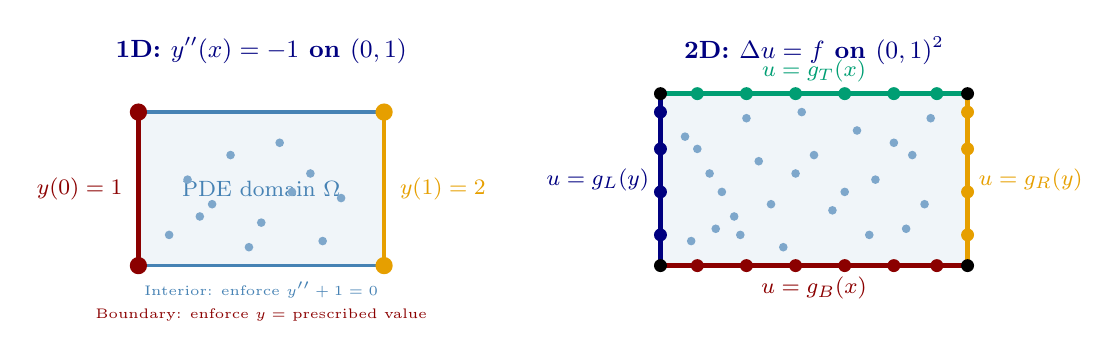
\begin{tikzpicture}[scale=0.78]
    % --- 1D example (left) ---
    \begin{scope}[shift={(-5.5,0)}]
        \node[font=\small\bfseries, uzhblue] at (2,3.5) {1D: $y''(x) = -1$ on $(0,1)$};

        % Domain line
        \draw[very thick, softblue, fill=softblue!8] (0,0) rectangle (4,2.5);
        \node[font=\footnotesize, softblue] at (2,1.25) {PDE domain $\Omega$};

        % Left boundary
        \draw[ultra thick, darkred] (0,0) -- (0,2.5);
        \node[left, font=\footnotesize, darkred] at (-0.1,1.25) {$y(0)=1$};
        \fill[darkred] (0,0) circle (4pt);
        \fill[darkred] (0,2.5) circle (4pt);

        % Right boundary
        \draw[ultra thick, softorange] (4,0) -- (4,2.5);
        \node[right, font=\footnotesize, softorange] at (4.1,1.25) {$y(1)=2$};
        \fill[softorange] (4,0) circle (4pt);
        \fill[softorange] (4,2.5) circle (4pt);

        % Interior collocation dots
        \foreach \pt in {{0.5,0.5},{1.2,1.0},{2.0,0.7},{2.8,1.5},{1.5,1.8},
            {3.0,0.4},{0.8,1.4},{2.3,2.0},{3.3,1.1},{1.0,0.8},{2.5,1.2},{1.8,0.3}}{
            \fill[softblue!70] (\pt) circle (2pt);
        }
        \node[font=\tiny, softblue] at (2,-0.4) {Interior: enforce $y''+1=0$};
        \node[font=\tiny, darkred] at (2,-0.8) {Boundary: enforce $y=$ prescribed value};
    \end{scope}

    % --- 2D example (right) ---
    \begin{scope}[shift={(3.0,0)}]
        \node[font=\small\bfseries, uzhblue] at (2.5,3.5) {2D: $\Delta u = f$ on $(0,1)^2$};

        % Domain
        \fill[softblue!8] (0,0) rectangle (5,2.8);

        % Boundary sides with different colors
        \draw[ultra thick, darkred] (0,0) -- (5,0)
            node[midway, below, font=\footnotesize] {$u = g_B(x)$};
        \draw[ultra thick, softorange] (5,0) -- (5,2.8)
            node[midway, right, font=\footnotesize] {$u = g_R(y)$};
        \draw[ultra thick, softgreen] (0,2.8) -- (5,2.8)
            node[midway, above, font=\footnotesize] {$u = g_T(x)$};
        \draw[ultra thick, uzhblue] (0,0) -- (0,2.8)
            node[midway, left, font=\footnotesize] {$u = g_L(y)$};

        % Interior points
        \foreach \pt in {{0.5,0.4},{1.2,0.8},{2.0,0.3},{3.0,1.2},{4.0,0.6},
            {0.8,1.5},{1.8,1.0},{2.5,1.8},{3.5,1.4},{4.3,1.0},
            {0.4,2.1},{1.4,2.4},{2.2,1.5},{3.2,2.2},{4.1,1.8},
            {0.9,0.6},{1.6,1.7},{2.8,0.9},{3.8,2.0},{1.0,1.2},
            {2.3,2.5},{3.4,0.5},{4.4,2.4},{0.6,1.9},{1.3,0.5}}{
            \fill[softblue!70] (\pt) circle (2pt);
        }

        % Boundary points
        \foreach \rt in {0.6,1.4,2.2,3.0,3.8,4.5}{
            \fill[darkred] (\rt,0) circle (3pt);
            \fill[softgreen] (\rt,2.8) circle (3pt);
        }
        \foreach \rt in {0.5,1.2,1.9,2.5}{
            \fill[uzhblue] (0,\rt) circle (3pt);
            \fill[softorange] (5,\rt) circle (3pt);
        }

        % Corner markers
        \fill[black] (0,0) circle (3pt);
        \fill[black] (5,0) circle (3pt);
        \fill[black] (0,2.8) circle (3pt);
        \fill[black] (5,2.8) circle (3pt);
    \end{scope}
\end{tikzpicture}
\end{center}

\vspace{0.2em}
\begin{block}{Two enforcement strategies}
\textbf{Soft:} add BC violation as a penalty term in the loss.\\
\textbf{Hard:} build BCs into the network output by construction.
\end{block}
\end{frame}

% --- Slide 19c: Visual: Soft BC Problems ---
\begin{frame}{The Problem with Soft Boundary Conditions}
\begin{center}
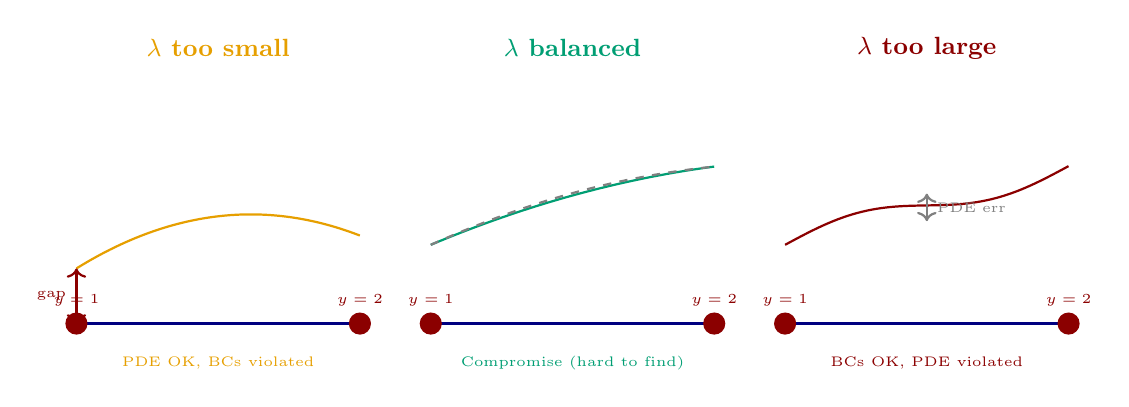
\begin{tikzpicture}
    % Three scenarios
    % Lambda too small
    \begin{scope}[shift={(-5,0)}]
        \node[font=\small\bfseries, softorange] at (1.8,3.5) {$\lambda$ too small};
        \draw[thick, uzhblue] (0,0) -- (3.6,0);
        \fill[darkred] (0,0) circle (4pt);
        \fill[darkred] (3.6,0) circle (4pt);
        \node[above, font=\tiny, darkred] at (0,0.1) {$y=1$};
        \node[above, font=\tiny, darkred] at (3.6,0.1) {$y=2$};
        % Solution that misses BCs
        \draw[thick, softorange, domain=0:3.6, samples=60]
            plot (\x, {-0.14*\x*\x + 0.62*\x + 0.7});
        \node[font=\tiny, softorange] at (1.8,-0.5) {PDE OK, BCs violated};
        % Show BC mismatch
        \draw[thick, darkred, <->] (0,0) -- (0,0.7) node[midway, left, font=\tiny] {gap};
    \end{scope}

    % Lambda balanced
    \begin{scope}[shift={(-0.5,0)}]
        \node[font=\small\bfseries, softgreen] at (1.8,3.5) {$\lambda$ balanced};
        \draw[thick, uzhblue] (0,0) -- (3.6,0);
        \fill[darkred] (0,0) circle (4pt);
        \fill[darkred] (3.6,0) circle (4pt);
        \node[above, font=\tiny, darkred] at (0,0.1) {$y=1$};
        \node[above, font=\tiny, darkred] at (3.6,0.1) {$y=2$};
        % Good solution
        \draw[thick, softgreen, domain=0:3.6, samples=60]
            plot (\x, {-0.04*\x*\x + 0.42*\x + 1.0});
        % Analytical for reference (dashed)
        \draw[thick, dashed, gray, domain=0:3.6, samples=60]
            plot (\x, {-0.04*\x*\x + 0.42*\x + 1.0 + 0.03*sin(deg(3.14*\x/3.6))});
        \node[font=\tiny, softgreen] at (1.8,-0.5) {Compromise (hard to find)};
    \end{scope}

    % Lambda too large
    \begin{scope}[shift={(4,0)}]
        \node[font=\small\bfseries, darkred] at (1.8,3.5) {$\lambda$ too large};
        \draw[thick, uzhblue] (0,0) -- (3.6,0);
        \fill[darkred] (0,0) circle (4pt);
        \fill[darkred] (3.6,0) circle (4pt);
        \node[above, font=\tiny, darkred] at (0,0.1) {$y=1$};
        \node[above, font=\tiny, darkred] at (3.6,0.1) {$y=2$};
        % Solution that nails BCs but bad interior
        \draw[thick, darkred, domain=0:3.6, samples=60]
            plot (\x, {1.0 + \x/3.6 + 0.15*sin(deg(2*3.14*\x/3.6))});
        \node[font=\tiny, darkred] at (1.8,-0.5) {BCs OK, PDE violated};
        % Show interior wiggle
        \draw[thick, gray, <->] (1.8,1.3) -- (1.8,1.65) node[midway, right, font=\tiny] {PDE err};
    \end{scope}
\end{tikzpicture}
\end{center}

\vspace{0.4em}
\begin{center}
{\small Soft BCs require \emphc{careful balancing} of the penalty weight $\lambda$.\\
Too small: BCs violated. Too large: PDE ignored. Just right: hard to find \emph{a priori}.}
\end{center}
\end{frame}

% --- Slide 20: Hard BC Trial Solution ---
\begin{frame}{Hard BC Enforcement: Trial Solutions}
\textbf{Idea:} construct a \emphc{trial solution} that satisfies BCs \emph{by construction}:
\[
\boxed{
\hat{y}(x) = A(x) + B(x)\cdot\mathcal{N}_\theta(x)
}
\]

\vspace{0.2em}
where:
\begin{itemize}
    \item $A(x)$: \emphc{anchor function} satisfying the BCs exactly, e.g.\ $A(x) = 1 + x$
    \item $B(x)$: \emphc{mask function} vanishing at boundaries, e.g.\ $B(x) = x(1-x)$
    \item $\mathcal{N}_\theta(x)$: free neural network (no BC constraints)
\end{itemize}

\vspace{0.3em}
\textbf{Verification:}
\begin{align*}
\hat{y}(0) &= A(0) + B(0)\cdot\mathcal{N}_\theta(0) = 1 + 0 = 1 \quad\checkmark\\
\hat{y}(1) &= A(1) + B(1)\cdot\mathcal{N}_\theta(1) = 2 + 0 = 2 \quad\checkmark
\end{align*}

$\Rightarrow$ BCs hold \emphc{identically}---only the PDE residual loss remains.
\end{frame}

% --- Slide 20b: Trial Solution Visual Decomposition ---
\begin{frame}{Trial Solution: Visual Decomposition}
\vspace{-0.3em}
\begin{center}
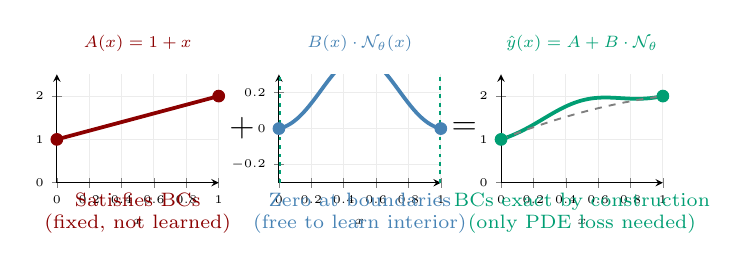
\begin{tikzpicture}[scale=0.85]
    % A(x) plot
    \begin{axis}[
        name=plotA,
        width=4.0cm, height=3.2cm,
        title={\scriptsize $A(x) = 1 + x$},
        title style={font=\scriptsize\bfseries, text=darkred},
        xlabel={$x$}, xlabel style={font=\tiny},
        ylabel style={font=\tiny},
        tick label style={font=\tiny},
        xmin=0, xmax=1, ymin=0, ymax=2.5,
        grid=major, grid style={gray!15},
        axis lines=left,
    ]
        \addplot[ultra thick, darkred, domain=0:1, samples=2]{1+x};
        \addplot[only marks, mark=*, mark size=2.5pt, darkred]
            coordinates {(0,1) (1,2)};
    \end{axis}

    % Plus sign
    \node[font=\large\bfseries] at ($(plotA.east)+(0.35,0)$) {$+$};

    % B(x) * N(x) plot
    \begin{axis}[
        at={($(plotA.east)+(0.9cm,0)$)}, anchor=west,
        name=plotBN,
        width=4.0cm, height=3.2cm,
        title={\scriptsize $B(x)\cdot\mathcal{N}_\theta(x)$},
        title style={font=\scriptsize\bfseries, text=softblue},
        xlabel={$x$}, xlabel style={font=\tiny},
        ylabel style={font=\tiny},
        tick label style={font=\tiny},
        xmin=0, xmax=1, ymin=-0.3, ymax=0.3,
        grid=major, grid style={gray!15},
        axis lines=left,
    ]
        \addplot[ultra thick, softblue, domain=0:1, samples=80]
            {x*(1-x)*(0.8*sin(deg(3.14*x)) - 0.3*cos(deg(2*3.14*x)) + 0.5)};
        \addplot[only marks, mark=*, mark size=2.5pt, softblue]
            coordinates {(0,0) (1,0)};
        \draw[ultra thick, softgreen, dotted] (axis cs:0,-0.3) -- (axis cs:0,0.3);
        \draw[ultra thick, softgreen, dotted] (axis cs:1,-0.3) -- (axis cs:1,0.3);
    \end{axis}

    % Equals sign
    \node[font=\large\bfseries] at ($(plotBN.east)+(0.35,0)$) {$=$};

    % y_hat(x) plot
    \begin{axis}[
        at={($(plotBN.east)+(0.9cm,0)$)}, anchor=west,
        name=plotY,
        width=4.0cm, height=3.2cm,
        title={\scriptsize $\hat{y}(x) = A + B\cdot\mathcal{N}_\theta$},
        title style={font=\scriptsize\bfseries, text=softgreen},
        xlabel={$x$}, xlabel style={font=\tiny},
        ylabel style={font=\tiny},
        tick label style={font=\tiny},
        xmin=0, xmax=1, ymin=0, ymax=2.5,
        grid=major, grid style={gray!15},
        axis lines=left,
    ]
        \addplot[ultra thick, softgreen, domain=0:1, samples=80]
            {1 + x + x*(1-x)*(0.8*sin(deg(3.14*x)) - 0.3*cos(deg(2*3.14*x)) + 0.5)};
        \addplot[thick, dashed, gray, domain=0:1, samples=80]
            {-0.5*x^2 + 1.5*x + 1};
        \addplot[only marks, mark=*, mark size=2.5pt, softgreen]
            coordinates {(0,1) (1,2)};
    \end{axis}

    % Annotations below -- use scriptsize to avoid overlap
    \node[font=\scriptsize, darkred, align=center] at ($(plotA.south)-(0,0.45)$)
        {Satisfies BCs\\(fixed, not learned)};
    \node[font=\scriptsize, softblue, align=center] at ($(plotBN.south)-(0,0.45)$)
        {Zero at boundaries\\(free to learn interior)};
    \node[font=\scriptsize, softgreen, align=center] at ($(plotY.south)-(0,0.45)$)
        {BCs exact by construction\\(only PDE loss needed)};
\end{tikzpicture}
\end{center}
\end{frame}

% --- Slide 21: Hard BC Code ---
\begin{frame}[fragile]{Hard BC: Implementation}
\begin{lstlisting}[basicstyle=\scriptsize\ttfamily]
def A(x):                          # Anchor: A(0)=1, A(1)=2
    return 1.0 + x
def B(x):                          # Mask: B(0)=B(1)=0
    return x * (1.0 - x)

def y_trial(model, x):            # Hard-BC trial solution
    return A(x) + B(x) * model(x)

def residual(model, x):
    x.requires_grad_(True)
    y = y_trial(model, x)
    dydx   = torch.autograd.grad(y, x, (*@\ldots@*))[0]
    d2ydx2 = torch.autograd.grad(dydx, x, (*@\ldots@*))[0]
    return d2ydx2 + 1.0           # should be 0
\end{lstlisting}

\vspace{0.2em}
{\small \textbf{Advantage:} the loss has \emphc{only one term} (PDE residual)---no $\lambda$ to tune!}
\end{frame}

% --- Slide 21b: Visual: 2D Hard BC Construction ---
\begin{frame}{Hard BCs in 2D: Building the Trial Solution}
\begin{center}
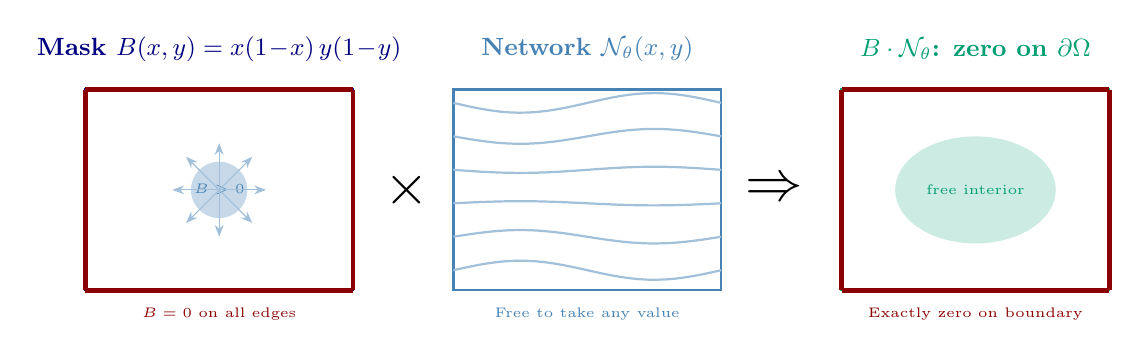
\begin{tikzpicture}[scale=0.85]
    % --- Mask B(x,y) ---
    \begin{scope}[shift={(-5.5,0)}]
        \node[font=\small\bfseries, uzhblue] at (2,3.6) {Mask $B(x,y) = x(1\!-\!x)\,y(1\!-\!y)$};
        % Domain square
        \draw[thick, uzhblue] (0,0) rectangle (4,3);
        % Zero on boundary (thick red)
        \draw[ultra thick, darkred] (0,0) -- (4,0);
        \draw[ultra thick, darkred] (4,0) -- (4,3);
        \draw[ultra thick, darkred] (4,3) -- (0,3);
        \draw[ultra thick, darkred] (0,3) -- (0,0);
        \node[font=\tiny, darkred] at (2,-0.35) {$B = 0$ on all edges};
        % Interior peak
        \fill[softblue!30] (2,1.5) circle (12pt);
        \node[font=\tiny, softblue] at (2,1.5) {$B > 0$};
        % Arrows showing B vanishes
        \foreach \a in {0,45,...,315}{
            \draw[-{Stealth[length=1.5mm]}, thin, softblue!50]
                (2,1.5) -- +(\a:0.7);
        }
    \end{scope}

    % Plus sign
    \node[font=\huge\bfseries] at (-0.7,1.5) {$\times$};

    % --- Network N(x,y) ---
    \begin{scope}[shift={(0,0)}]
        \node[font=\small\bfseries, softblue] at (2,3.6) {Network $\mathcal{N}_\theta(x,y)$};
        \draw[thick, softblue] (0,0) rectangle (4,3);
        % Wavy surface (NN output)
        \foreach \y in {0.3,0.8,...,2.8}{
            \draw[softblue!50, thick, domain=0:4, samples=30]
                plot (\x, {\y + 0.15*sin(deg(2*3.14*\x/4))*cos(deg(3.14*\y/3))});
        }
        \node[font=\tiny, softblue] at (2,-0.35) {Free to take any value};
    \end{scope}

    % Arrow to result
    \node[font=\huge\bfseries] at (4.8,1.5) {$\Rightarrow$};

    % --- Result B*N ---
    \begin{scope}[shift={(5.8,0)}]
        \node[font=\small\bfseries, softgreen] at (2,3.6) {$B \cdot \mathcal{N}_\theta$: zero on $\partial\Omega$};
        \draw[thick, softgreen] (0,0) rectangle (4,3);
        % Zero boundary (flat edges)
        \draw[ultra thick, darkred] (0,0) -- (4,0);
        \draw[ultra thick, darkred] (4,0) -- (4,3);
        \draw[ultra thick, darkred] (4,3) -- (0,3);
        \draw[ultra thick, darkred] (0,3) -- (0,0);
        % Interior variation (damped by B)
        \fill[softgreen!20] (2,1.5) ellipse (1.2 and 0.8);
        \node[font=\tiny, softgreen] at (2,1.5) {free interior};
        \node[font=\tiny, darkred] at (2,-0.35) {Exactly zero on boundary};
    \end{scope}
\end{tikzpicture}
\end{center}

\vspace{0.3em}
{\small Then $\hat{u}(x,y) = \underbrace{A(x,y)}_{\text{matches BCs}} + \underbrace{B(x,y)\cdot\mathcal{N}_\theta(x,y)}_{\text{zero on }\partial\Omega}$ satisfies Dirichlet BCs \emphc{exactly}.}
\end{frame}

% --- Slide 22: Soft vs Hard Comparison ---
\begin{frame}{Soft vs.\ Hard BCs: Comparison}
\begin{center}
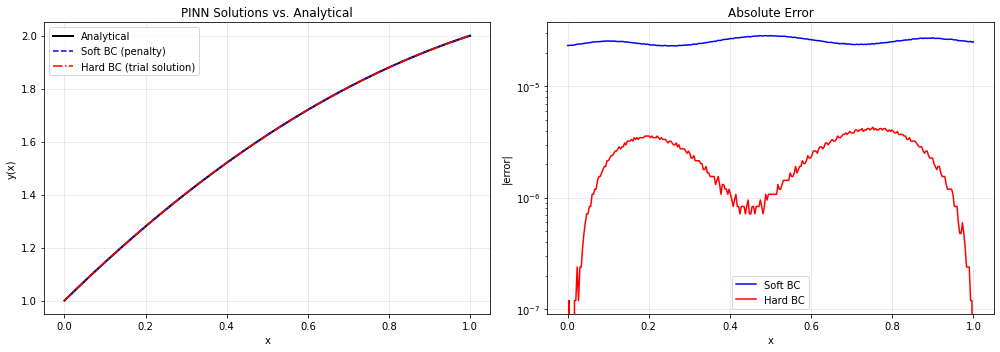
\includegraphics[width=0.90\linewidth]{fig/day6_ext/pinn_softvshard.png}
\end{center}

\vspace{0.05em}
\begin{center}
{\footnotesize Hard BCs eliminate boundary error by construction, so the optimizer only fits the PDE interior. The notebook compares this against the tuned soft-penalty baseline.}
\end{center}

{\footnotesize\hfill\textbf{Notebook:} \texttt{02\_ODE\_PINN\_SoftVsHardBCs}}
\end{frame}

% --- Finger Exercise: Hard BCs ---
\begin{frame}{\exercisepause{} Finger Exercise: Hard Boundary Conditions}
\begin{exampleblock}{Exercise (5 min)}
Consider the same ODE $u''(x) = -1$ on $[0,1]$ with $u(0)=u(1)=0$.
\begin{enumerate}
    \item Construct a \emphc{hard-BC trial solution} of the form $\hat{u}(x) = B(x) \cdot \mathcal{N}(x; \theta)$, where $B(x)$ enforces both BCs exactly. {\small (Hint: $B$ must vanish at $x=0$ and $x=1$.)}
    \item Verify that $\hat{u}(0) = \hat{u}(1) = 0$ for \emph{any} network output $\mathcal{N}$.
    \item What is the advantage of hard BCs over soft BCs?
\end{enumerate}
\end{exampleblock}
\end{frame}

\begin{frame}{Solution: Hard Boundary Conditions}
\begin{block}{Answer}
\begin{enumerate}
    \item $\hat{u}(x) = x(1-x)\cdot\mathcal{N}(x; \theta)$.  Since $B(x)=x(1-x)$ vanishes at both endpoints, the BCs are satisfied exactly.
    \item $\hat{u}(0)=0\cdot\mathcal{N}(0;\theta)=0$. \quad $\hat{u}(1)=0\cdot\mathcal{N}(1;\theta)=0$. \checkmark\\
    This holds regardless of what $\mathcal{N}$ outputs.
    \item Hard BCs \emphc{eliminate the boundary loss term} entirely---the optimizer only needs to minimize the PDE residual. This reduces the number of hyperparameters ($\lambda$ is gone) and often speeds up convergence.
\end{enumerate}
\end{block}
\end{frame}

% --- Slide 23: 2D Poisson ---
\begin{frame}{Extension to 2D: Poisson Equation}
\textbf{Problem:} $\Delta u = f(x,y)$ on $\Omega = (0,1)^2$ with Dirichlet BCs.

\vspace{0.2em}
\textbf{Manufactured solution:} $u^\star(x,y) = x^2 + y + \sin(\pi x)\sin(\pi y)$.

\vspace{0.4em}
\textbf{Hard BCs via transfinite (Coons-patch) interpolation} --- the standard 4-side construction that matches each boundary function exactly along its edge:
\[
\hat{u}(x,y) = A(x,y) + \underbrace{x(1\!-\!x)\,y(1\!-\!y)}_{B(x,y)}\cdot\mathcal{N}_\theta(x,y)
\]

where $A(x,y)$ interpolates boundary data from all four sides:
\[
A = (1\!-\!x)\,g_L(y) + x\,g_R(y) + (1\!-\!y)\,g_B(x) + y\,g_T(x) - \text{corners}
\]

\vspace{0.3em}
\textbf{Laplacian via autograd:}
\[
\Delta\hat{u} = \frac{\partial^2\hat{u}}{\partial x^2} + \frac{\partial^2\hat{u}}{\partial y^2}
\quad\text{(two chains of \texttt{autograd.grad})}
\]
\end{frame}

% --- Slide 24: 2D Results ---
\begin{frame}{2D Poisson: Results}
\begin{center}
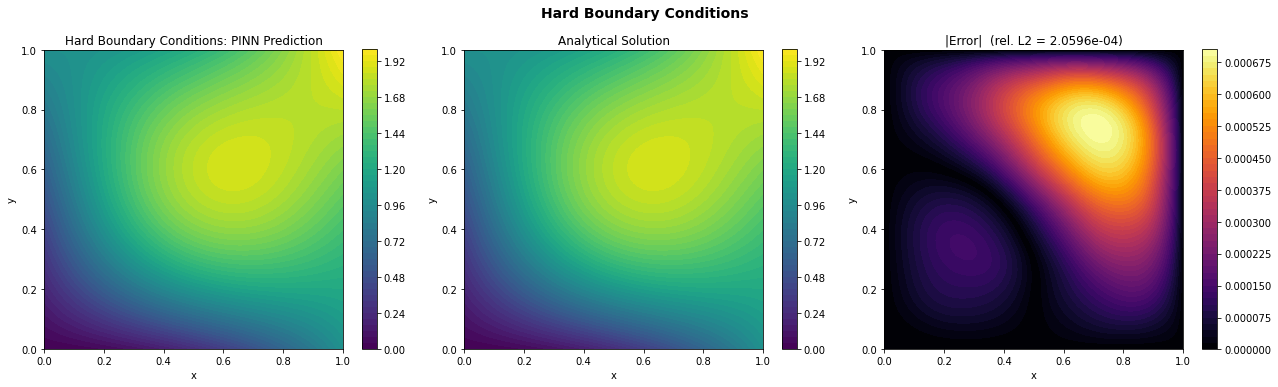
\includegraphics[width=0.96\linewidth]{fig/day6_ext/pinn_poisson2d_hard.png}
\end{center}

\vspace{0.1em}
\begin{center}
{\small Hard-BC PINN, analytical solution, and absolute error.\\Relative $L^2$ error $\approx 2.06\times 10^{-4}$. Boundary conditions satisfied \emphc{exactly}.}
\end{center}

{\small\hfill\textbf{Notebook:} \texttt{03\_PDE\_PINN\_Poisson2D}}
\end{frame}

% --- Slide 25: When to Use Which ---
\begin{frame}{Soft vs.\ Hard BCs: When to Use Which?}
\begin{center}
{\small
\begin{tabular}{p{2.2cm}p{4.5cm}p{4.5cm}}
\toprule
& \textbf{Soft BCs} & \textbf{Hard BCs} \\
\midrule
\textbf{Best for} & Complex geometries, time-dependent BCs, Robin/Neumann & Simple domains, Dirichlet BCs, high accuracy \\
\midrule
\textbf{Pros} & Flexible, easy to implement & Exact BCs, fewer hyperparams, better accuracy \\
\midrule
\textbf{Cons} & $\lambda$ tuning, approximate BCs & Needs analytical $A$, $B$; harder for irregular domains \\
\bottomrule
\end{tabular}
}
\end{center}

\vspace{0.3em}
\begin{block}{Practical recommendation}
Start with \emphc{hard BCs} when the domain and boundary data allow it.
Fall back to \emphc{soft BCs} for complex geometries or mixed boundary types.
\end{block}
\end{frame}

% ============================================================================
% PART IV: ECONOMIC APPLICATIONS --- HJB
% ============================================================================

% --- Slide 26: Section Divider ---
\begin{frame}{}
\vfill
\begin{center}
{\Huge \textcolor{uzhblue}{\textbf{Part IV}}}\\[12pt]
{\LARGE Economic Applications: The HJB Equation}
\end{center}
\vfill
\end{frame}

% --- Slide 27: HJB Equation ---
\begin{frame}{The Hamilton--Jacobi--Bellman Equation}
\textbf{Generic continuous-time optimization:}
\[
\rho\, V(\x) = \max_{c}\;\bigl\{u(c) + V_{\x}\cdot f(\x, c)\bigr\}
\]

\vspace{0.3em}
\begin{itemize}
    \item $V(\x)$: \emphc{value function} (unknown)
    \item $\rho$: discount rate
    \item $u(c)$: flow utility
    \item $f(\x,c)$: law of motion for state $\x$
    \item $V_{\x} = \nabla V$: gradient of the value function
\end{itemize}

\vspace{0.4em}
\textbf{This is a PDE!} First-order (or second-order with diffusion).

\vspace{0.3em}
$\Rightarrow$ \emphc{Perfect fit for PINNs:} the network approximates $V$, autograd gives $V_{\x}$, and the HJB residual is the loss.
\end{frame}

% --- Slide 28: Cake-Eating Setup ---
\begin{frame}{Cake-Eating Problem: Setup}
\textbf{A household} chooses consumption $c(t)$ to maximize lifetime utility:
\[
\max_{\{c(t)\}} \int_0^\infty e^{-\rho t}\,\frac{c(t)^{1-\gamma}}{1-\gamma}\,\mathrm{d}t
\qquad\text{s.t.}\quad \dot{a} = r\,a - c
\]

\textbf{HJB equation:}\quad
$\rho\,V(a) = \max_c\;\bigl\{\frac{c^{1-\gamma}}{1-\gamma} + V'(a)\,(r\,a - c)\bigr\}$

\vspace{0.2em}
\textbf{FOC:} $c^{-\gamma} = V'(a)$ $\;\Rightarrow\;$ $c^\star = \bigl(V'(a)\bigr)^{-1/\gamma}$.

\vspace{0.2em}
\textbf{Analytical solution} (with $\kappa = \frac{\rho - (1-\gamma)r}{\gamma} > 0$):
\[
V^\star(a) = \frac{\kappa^{-\gamma}}{1-\gamma}\,a^{1-\gamma}, \qquad c^\star(a) = \kappa\,a
\]

{\small Parameters: $\gamma = 2$, $\rho = 0.05$, $r = 0.03$ $\;\Rightarrow\;$ $\kappa = 0.04$.}
\end{frame}

% --- Slide 29: PINN for HJB (trial solution, hard BCs) ---
\begin{frame}{PINN for the HJB Equation: Hard-BC Trial Solution}
\textbf{Anchor + mask + scaled MLP.}  Let $x(a) = (a-a_{\min})/(a_{\max}-a_{\min}) \in [0,1]$ and $S$ a value-scale constant:
\[
\hat V(a) \;=\; V^\star(a_{\min}) + x(a)\bigl[V^\star(a_{\max}) - V^\star(a_{\min})\bigr] \;+\; x(a)\bigl(1-x(a)\bigr)\,S\,f_\theta\bigl(x(a)\bigr).
\]
Endpoints are exact \emph{by construction}, so the boundary loss is identically zero and the optimizer focuses on the HJB residual only.

\vspace{0.3em}
\textbf{Consumption} via FOC, $\hat c(a) = (\hat V'(a))^{-1/\gamma}$, with softplus safeguard on $\hat V'$.

\vspace{0.3em}
\textbf{Loss}: only the interior HJB residual remains,
\[
\ell \;=\; \frac{1}{N}\sum_{i}\mathcal{R}(a_i)^2,
\qquad
\mathcal{R}(a) = \rho\hat V - \Bigl[\tfrac{\hat c^{1-\gamma}}{1-\gamma} + \hat V'(ra - \hat c)\Bigr].
\]

\vspace{0.2em}
{\small \emphc{Pedagogical point:} a small MLP plus hard BCs beats a large gated net with a soft-BC penalty, because the boundary term no longer dominates the objective.}
\end{frame}

% --- Slide 30: DGM Architecture (optional / high-D) ---
\begin{frame}[shrink=15]{Optional Architecture for High-D PDEs: DGM}
\begin{columns}[T]
\column{0.40\textwidth}
{\small\textbf{Deep Galerkin Method} (Sirignano \& Spiliopoulos, 2018) --- a heavier architecture that becomes worth its weight only in higher dimensions or with sharp PDE features.  For the 1D cake problem, the trial-solution MLP on the previous slide is preferred.}

\vspace{0.3em}
\begin{center}
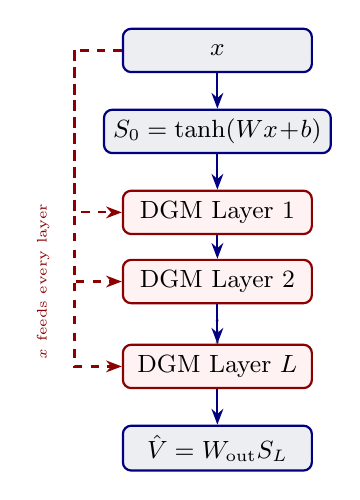
\begin{tikzpicture}[
    block/.style={rectangle, draw=uzhblue, thick, fill=uzhgreylight,
        minimum width=2.4cm, minimum height=0.55cm, font=\small,
        rounded corners=3pt},
    layer/.style={rectangle, draw=darkred, thick, fill=red!5,
        minimum width=2.4cm, minimum height=0.55cm, font=\small,
        rounded corners=3pt},
    arr/.style={-{Stealth[length=2mm]}, thick, uzhblue},
    skip/.style={-{Stealth[length=2mm]}, thick, darkred, dashed}
]
    % Input
    \node[block] (inp) {$x$};

    % Initial transform
    \node[block, below=0.45cm of inp] (S0) {$S_0 = \tanh(Wx\!+\!b)$};

    % DGM Layers — stacked to show repetition
    \node[layer, below=0.45cm of S0] (L1) {DGM Layer 1};
    \node[layer, below=0.3cm of L1] (L2) {DGM Layer 2};
    \node[font=\large, text=gray] at ($(L2.south)+(0,-0.25)$) {$\vdots$};
    \node[layer, below=0.5cm of L2] (LL) {DGM Layer $L$};

    % Output
    \node[block, below=0.45cm of LL] (out) {$\hat{V} = W_{\text{out}} S_L$};

    % Vertical arrows
    \draw[arr] (inp) -- (S0);
    \draw[arr] (S0) -- (L1);
    \draw[arr] (L1) -- (L2);
    \draw[arr] (L2) -- (LL);
    \draw[arr] (LL) -- (out);

    % Skip connections from x to every layer
    \draw[skip] (inp.west) -- ++(-0.6,0) |- (L1.west);
    \draw[skip] ([xshift=-0.6cm]inp.west) |- (L2.west);
    \draw[skip] ([xshift=-0.6cm]inp.west) |- (LL.west);

    % Label for skip connections
    \node[font=\tiny, text=darkred, align=center, rotate=90]
        at ([xshift=-1.0cm]L2.west) {$x$ feeds every layer};
\end{tikzpicture}
\end{center}

\column{0.58\textwidth}
{\footnotesize \textcolor{darkred}{\textbf{DGM Layer}} \emphc{gates} (LSTM-like, Hochreiter \& Schmidhuber 1997); $x$-skip connections recall Highway Networks (Srivastava et al.\ 2015). $S_\ell\in\R^U$ is the depth-$\ell$ hidden state ($S_0=\tanh(Wx+b)$), $\odot$ is Hadamard, $Z,G,R$ are sigmoid gates in $[0,1]$:}
\vspace{-0.6em}
{\footnotesize\begin{align*}
Z_\ell &= \sigma(U^z x + W^z S_\ell + b^z)\\
G_\ell &= \sigma(U^g x + W^g S_\ell + b^g)\\
R_\ell &= \sigma(U^r x + W^r S_\ell + b^r)\\
H_\ell &= \tanh(U^h x + W^h (S_\ell \odot R_\ell) + b^h)\\
S_{\ell+1} &= (1 - G_\ell)\odot H_\ell + Z_\ell \odot S_\ell
\end{align*}}
\vspace{-1.0em}

{\footnotesize \textbf{Key idea:} feeding $x$ into every layer helps the network resolve sharp PDE gradients.}
\end{columns}
\end{frame}

% --- Slide 31: DGM Code ---
\begin{frame}[fragile]{DGM Implementation (PyTorch)}
\begin{lstlisting}[basicstyle=\scriptsize\ttfamily]
class DGMNet(nn.Module):
    def __init__(self, dim, layers=4, units=64):
        super().__init__()
        self.input = nn.Linear(dim, units)
        self.z  = nn.ModuleList(nn.Linear(dim, units) for _ in range(layers))
        self.wz = nn.ModuleList(nn.Linear(units, units) for _ in range(layers))
        # ... similar for g, r, h gates
        self.out = nn.Linear(units, 1)

    def forward(self, x):
        s = torch.tanh(self.input(x))
        for l in range(len(self.z)):
            z = torch.sigmoid(self.z[l](x) + self.wz[l](s))
            g = torch.sigmoid(self.g[l](x) + self.wg[l](s))
            r = torch.sigmoid(self.r[l](x) + self.wr[l](s))
            h = torch.tanh(self.h[l](x) + self.wh[l](s * r))
            s = (1 - g) * h + z * s
        return self.out(s)
\end{lstlisting}
\end{frame}

% --- Slide 32: HJB Residual Code ---
\begin{frame}[fragile]{HJB Residual Implementation}
\begin{lstlisting}[basicstyle=\footnotesize\ttfamily]
def pde_residual(model, a):
    a.requires_grad_(True)
    V = model(a)                        # value function
    V_a = torch.autograd.grad(          # V'(a) via autograd
        V.sum(), a, create_graph=True)[0].squeeze(-1)

    safe_Va = F.softplus(V_a) + 1e-6   # positivity guard
    c = safe_Va.pow(-1.0 / gamma)       # FOC: optimal c
    u_c = c.pow(1-gamma) / (1-gamma)    # flow utility

    R = rho*V - (u_c + safe_Va*(r*a.squeeze(-1) - c))
    return R                            # HJB residual
\end{lstlisting}

\vspace{0.1em}
{\footnotesize The \texttt{softplus} safeguard prevents $V'(a)^{-1/\gamma}$ from blowing up if $V'(a) \leq 0$ during early training.}
\end{frame}

% --- Slide 33: Cake-Eating Results ---
\begin{frame}{Cake-Eating: Expected Behavior (Schematic)}
\begin{columns}[T]
\column{0.48\textwidth}
\begin{center}
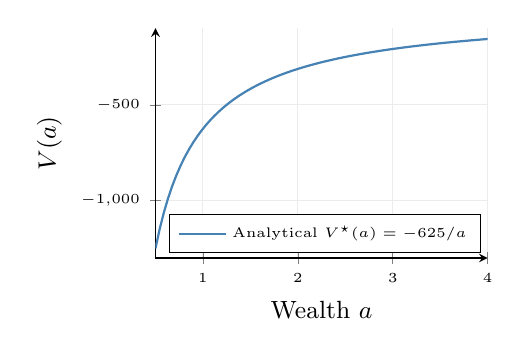
\begin{tikzpicture}
\begin{axis}[
    width=5.8cm, height=4.5cm,
    xlabel={Wealth $a$}, ylabel={$V(a)$},
    xlabel style={font=\small}, ylabel style={font=\small},
    tick label style={font=\tiny},
    xmin=0.5, xmax=4, ymin=-1300, ymax=-100,
    grid=major, grid style={gray!15},
    legend style={font=\tiny, at={(0.98,0.02)}, anchor=south east},
    axis lines=left,
]
    \addplot[thick, softblue, domain=0.5:4, samples=80] {-625/x};
    \addlegendentry{Analytical $V^\star(a) = -625/a$}
\end{axis}
\end{tikzpicture}\\
{\small Value function $V(a)$ (closed form)}
\end{center}

\column{0.48\textwidth}
\begin{center}
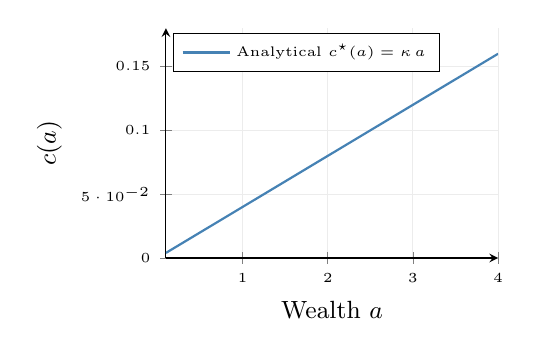
\begin{tikzpicture}
\begin{axis}[
    width=5.8cm, height=4.5cm,
    xlabel={Wealth $a$}, ylabel={$c(a)$},
    xlabel style={font=\small}, ylabel style={font=\small},
    tick label style={font=\tiny},
    xmin=0.1, xmax=4, ymin=0, ymax=0.18,
    grid=major, grid style={gray!15},
    legend style={font=\tiny, at={(0.02,0.98)}, anchor=north west},
    axis lines=left,
]
    \addplot[thick, softblue, domain=0.1:4, samples=80] {0.04*x};
    \addlegendentry{Analytical $c^\star(a) = \kappa\, a$}
\end{axis}
\end{tikzpicture}\\
{\small Consumption policy $c(a)$ (closed form)}
\end{center}
\end{columns}

\vspace{0.1em}
\begin{center}
{\footnotesize \emph{Validation target:} closed form. Classroom run: final HJB loss $\approx 3\!\times\!10^{-4}$; consumption relative $L^2$ error $\approx 6\!\times\!10^{-3}$ after Adam + FP64 L-BFGS.}
\end{center}

{\small\hfill\textbf{Notebook:} \texttt{04\_Cake\_Eating\_HJB\_PINN}}
\end{frame}

% --- Slide 34: Extensions ---
\begin{frame}{Extensions: From Cake-Eating to Frontier Models}
\textbf{The PINN/DGM framework scales naturally:}

\vspace{0.3em}
\begin{enumerate}
    \item \textbf{Income risk:} add diffusion $\mathrm{d}a = (ra - c + y)\,\mathrm{d}t + \sigma\,\mathrm{d}W$
    \quad$\Rightarrow$ second-order HJB

    \vspace{0.2em}
    \item \textbf{Aiyagari-type models:} HJB + Kolmogorov Forward Equation
    \quad$\Rightarrow$ coupled PDE system

    \vspace{0.2em}
    \item \textbf{General equilibrium:} prices clear markets
    \quad$\Rightarrow$ hybrid DEQN + PINN

    \vspace{0.2em}
    \item \textbf{High dimensions:} multiple assets, heterogeneous agents
    \quad$\Rightarrow$ no grid needed!
\end{enumerate}

\vspace{0.3em}
{\small See: Achdou et al.\ (2022), Fernandez-Villaverde et al.\ (2024), Gopalakrishna (2024).}
\end{frame}

% ============================================================================
% PART V: BLACK-SCHOLES
% ============================================================================

% --- Slide 35: Section Divider ---
\begin{frame}{}
\vfill
\begin{center}
{\Huge \textcolor{uzhblue}{\textbf{Part V}}}\\[12pt]
{\LARGE Financial Applications: Black--Scholes}
\end{center}
\vfill
\end{frame}

% --- Slide 36: Black-Scholes PDE ---
\begin{frame}{The Black--Scholes PDE}
\begin{columns}[T]
\column{0.52\textwidth}
\textbf{European call option} ($S$: asset, $K$: strike, $T$: maturity):
\[
\frac{\partial V}{\partial t} + \frac{1}{2}\sigma^2 S^2 \frac{\partial^2 V}{\partial S^2}
+ r S\frac{\partial V}{\partial S} - rV = 0
\]

\textbf{Terminal:} $V(S, T) = \max(S - K, 0)$

\textbf{Boundary conditions:}
\begin{itemize}\setlength{\itemsep}{1pt}
    \item $V(0, t) = 0$
    \item $V(S_{\max}, t) = S_{\max} - Ke^{-r(T-t)}$
\end{itemize}

\column{0.45\textwidth}
\textbf{PINN approach:}
\begin{itemize}\setlength{\itemsep}{2pt}
    \item Network $\mathcal{N}_\theta(S, t) \approx V(S, t)$
    \item Autograd: $V_t$, $V_S$, $V_{SS}$
    \item 4 loss terms:
\end{itemize}

\vspace{0.2em}
{\small
\begin{tabular}{rl}
$\ell_{\text{PDE}}$ & interior residual\\
$\ell_{\text{BC}_0}$ & $V(0,t) = 0$\\
$\ell_{\text{term}}$ & $V(S,T) = \text{payoff}$\\
$\ell_{\text{BC}_{S_{\max}}}$ & far-field BC\\
\end{tabular}
}
\end{columns}
\end{frame}

% --- Slide 37: Black-Scholes Implementation ---
\begin{frame}[fragile]{Black--Scholes PINN: Key Code}
\begin{lstlisting}
def pde_residual(model, S, t):
    S.requires_grad_(True)
    t.requires_grad_(True)
    X = torch.cat([S, t], dim=1)
    V = model(X)

    V_t  = torch.autograd.grad(V, t, (*@\ldots@*))[0]
    V_S  = torch.autograd.grad(V, S, (*@\ldots@*))[0]
    V_SS = torch.autograd.grad(V_S, S, (*@\ldots@*))[0]

    # Black-Scholes PDE residual
    res = V_t + 0.5*sigma**2*S**2*V_SS + r*S*V_S - r*V
    return res
\end{lstlisting}

\vspace{0.1em}
{\small\textbf{Loss:}
\[
\ell = \text{MSE}(\text{res}) + \text{MSE}(V|_{S=0}) + \text{MSE}(V|_{t=T} - \text{payoff}) + \text{MSE}(V|_{S_{\max}} - \text{target})
\]
}
\end{frame}

% --- Slide 38: Black-Scholes Results ---
\begin{frame}{Black--Scholes: Expected Behavior (Schematic)}
\begin{columns}[T]
\column{0.55\textwidth}
\begin{center}
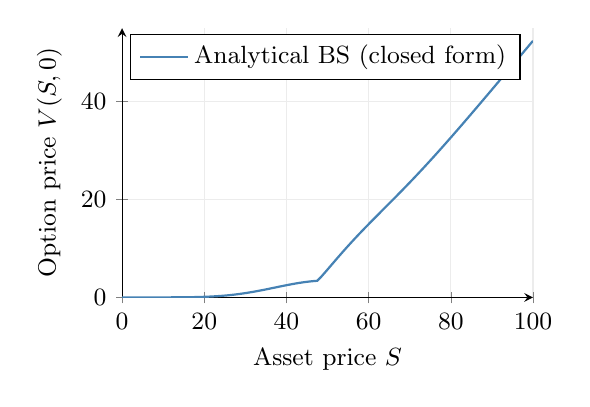
\begin{tikzpicture}
\begin{axis}[
    width=6.8cm, height=5cm,
    xlabel={Asset price $S$}, ylabel={Option price $V(S, 0)$},
    xlabel style={font=\small}, ylabel style={font=\small},
    tick label style={font=\small},
    xmin=0, xmax=100, ymin=0, ymax=55,
    grid=major, grid style={gray!15},
    legend style={font=\small, at={(0.02,0.98)}, anchor=north west},
    axis lines=left,
]
    \addplot[thick, softblue, domain=0:100, samples=100]
        {max(x - 50*exp(-0.05), 0) * 0.5*(1 + tanh(0.15*(x-42)))
         + 3.5*exp(-0.003*(x-50)^2) * 0.5*(1 + tanh(0.08*(x-20)))};
    \addlegendentry{Analytical BS (closed form)}
\end{axis}
\end{tikzpicture}
\end{center}

\column{0.42\textwidth}
{\small
\textbf{Parameters:} $K = 50$, $T = 1$, $r = 0.05$, $\sigma = 0.2$, $S_{\max} = 100$.

\vspace{0.2em}
\textbf{Network:} 3 hidden layers, 50 units, $\tanh$ activations, 10{,}000 epochs (Adam).

\vspace{0.3em}
\emph{Schematic} of the call-option price curve. Current notebook diagnostics report max absolute error $\approx 0.13$ and mean absolute error $\approx 0.04$ against the closed form.
}
\end{columns}

{\small\hfill\textbf{Notebook:} \texttt{05\_Black\_Scholes\_PINN}}
\end{frame}

% --- Slide 39: Summary ---
\begin{frame}{Summary and Key Takeaways}
\begin{columns}[T]
\column{0.32\textwidth}
\begin{block}{Method}
\centering\small
\vspace{0.2em}
PINNs embed \emphc{differential equations} directly into the neural network loss function via \emphc{automatic differentiation}.
\vspace{0.2em}
\end{block}

\column{0.32\textwidth}
\begin{block}{Boundary Conditions}
\centering\small
\vspace{0.2em}
\emphc{Hard BCs} (trial solutions) eliminate tuning and ensure exact satisfaction. Use \emphc{soft BCs} for complex domains.
\vspace{0.2em}
\end{block}

\column{0.32\textwidth}
\begin{block}{Applications}
\centering\small
\vspace{0.2em}
HJB equations, Black--Scholes, and any continuous-time model. Scales to \emphc{high dimensions} without grids.
\vspace{0.2em}
\end{block}
\end{columns}

\vspace{0.6em}
\textbf{From DEQNs to PINNs:}
\begin{itemize}
    \item \emphc{Same philosophy:} economic/financial equations \emph{are} the loss
    \item \emphc{New ingredient:} \texttt{torch.autograd.grad} for derivatives of $\mathcal{N}_\theta$
    \item \emphc{Broader scope:} any PDE, not just algebraic equilibrium conditions
\end{itemize}
\end{frame}

% --- Slide 40: Questions ---
\begin{frame}{}
\begin{columns}[c]
\column{0.45\textwidth}
\begin{center}
{\Huge \textcolor{uzhblue}{\textbf{Questions?}}}

\vspace{1.0cm}
{\large Simon Scheidegger}\\[4pt]
{\small HEC, University of Lausanne}\\[4pt]
\url{https://sischei.github.io}

\vspace{0.6cm}
{\small Materials:~~\url{https://github.com/sischei/Deep_Learning_for_Solving_And_Estimating_Dynamic_Economic_Models}}
\end{center}

\column{0.45\textwidth}
\begin{center}
\textbf{Companion Notebooks:}\\[8pt]
{\small
\begin{tabular}{rl}
01 & ODE PINN (Zero BCs) \\
02 & Soft vs.\ Hard BCs \\
03 & 2D Poisson \\
04 & Cake-Eating HJB \\
05 & Black--Scholes \\
\end{tabular}
}

\vspace{0.8cm}
\textbf{Next up (May 5th):}\\[6pt]
{\large Continuous-Time Heterogeneous}\\
{\large Agent Models: HJB + KFE}\\[8pt]
{\small 09:00--12:00}
\end{center}
\end{columns}
\end{frame}

\end{document}
